\chapter{Data}
\label{data}
\addcontentsline{toc}{chapter}{Data}

\section{Test Data}

We use data sets from the English-to-Czech Translation Task of the Workshop on
Statistical Machine Translation (WMT) from the years 2011 to 2014.

All of these datasets consist of one file with the original English source sentences,
several files with Czech hypotheses (outputs of MT systems) and one file with corresponding 
reference sentences. Data from each year of the WMT competition differ in the 
number of MT systems and the length of the source files (see \Tref{wmt-data}). 

%We perform morphological 
%analysis and tagging of the MT outputs and the reference sentences using 
%Morphodita \citep{morphodita}. \todo{nekde morphodita, nekde jeste morce}

\begin{table}[h]
\centering
\begin{tabular}{l|l|l|l|l}
      & systems & sentences & official score & publication\\
\hline
WMT11 & 14/10    & 3003      & “$ >= $ others”      & \cite{wmt11}  \\
WMT12 & 13          & 3003      & “$ > $ others”      & \cite{wmt12}  \\
WMT13 & 14/12    & 3000      & \textit{Expected Wins} & \cite{wmt13}  \\
WMT14 & 10          & 3003      & \textit{TrueSkill}   & \cite{wmt14}
\end{tabular}
\caption{Overview of WMT datasets. Number of systems translating from English 
to Czech (all MT systems / systems that were manually evaluated), number of 
source sentences and the official method for computing the absolute human 
judgement score.}
\label{wmt-data}
\end{table}

During the manual evaluation of WMT competitions, human judges fluent in both
the source and the target language scores five hypotheses from the best to
the worst translation. Thus, the human evaluation of hypotheses is available 
as~a~relative ranking of performance of five systems for~a~sentence. 

There are many ways to compute the absolute system score from this relative
ranking. The official methods for each year are presented in \Tref{wmt-data} 
and we refer to these as the \textit{gold standard}. The official method is
different for every year. Therefore, to make our evaluation internally 
consistent, we also compute another absolute score for every year using the 
“$ >$ others” method \citep{bojar-grains}, which was the WMT12 official system
score. This score is computed simply as $\frac{wins}{wins+loses} $, i.e., the 
score is~based on~how frequently the system is judged to be better than 
other systems, ties among several systems are ignored. We refer to this 
interpretation of human judgments as a \textit{silver standard} to distinguish
it from the official system scores. % todo: chcu to tu jeste zduvodnit, proc > others??

The performance of an evaluation metric in MT is commonly computed as the
Pearson correlation coefficient or alternatively as the Spearman rank 
correlation between the automatic metric and human judgment. 

The Pearson correlation coefficient $\rho$ is defined by the following formula:

\begin{equation*}
\rho(H,M) = \frac{ \sum_{i=1}^{n}{(H_i - \tilde{H})(M_i - \tilde{M})}}{ \sqrt{ \sum_{i=1}^{n}{(H_i - \tilde{H})^2} }  \sqrt{ \sum_{i=1}^{n}{(M_i - \tilde{M})^2} } } 
\end{equation*}

where $H$ is the vector of human scores (i.e. gold or silver standard here) and 
$M$ is the vector of corresponding scores predicted by a certain metric. 
$\tilde{H}$ a $\tilde{M}$ are their means, respectively. 

The Spearman correlation coefficient $r_{s} $ is defined as the Pearson 
correlation coefficient between the rank variables -- all human scores and  
metric’s scores of MT systems are converted into ranks $r(H)$ and $r(M)$.

\begin{equation*}
r_{s}(H,M) = \rho(r(H),r(M))
\end{equation*}

Both~correlations estimate the linear dependency between two sets of values and 
range from -1 (perfect negative linear relationship) to 1 (perfect linear correlation). 

In our experiments, we use the Pearson correlation coefficient as it takes into 
account the distances between the system scores, thus it should be more 
reliable for similarly evaluated systems \citep{machacek-bojar-2014-results}. 
\todo{tu to jeste trochu rozsirit, kdyz uz
to tu je vysvetleny - ze Spearman ignoruje jak moc jsou systemy od sebe vzdaleny}

%
%WMT13
%We measured the quality of system-level metrics’ scores using the Spearman’s rank correlation coefficient $\rho$. For each direction of translation we converted the official human scores into ranks. For each metric, we converted the metric’s scores of systems in a given direction into ranks. Since there were no ties in the rankings, we used the simplified formula to compute the Spearman’s $\rho$. 
%
%\begin{equation*}
%r_{s} = 1 -  \frac{6\sum{d_i^{2}}}{n(n^{2}-1)} 
%\end{equation*}
%where $d_{i}$ is the difference between the rank for system$_{i}$ and n is the number of systems. The possible values of range between 1 (where all systems are ranked in the same order) and -1 (where the systems are ranked in the reverse order). 
%
%\begin{equation*}
%r_{s} = r_{p}(r(H_{i}),r(M_{i}))
%\end{equation*}

\section{Sources of Czech Paraphrases}
We use the following available sources of Czech paraphrases.

\subsection{Czech WordNet}
Czech WordNet \citep{czech-wordnet} was created (by NLP Centre at the faculty of Informatics, Masaryk University ) as part of the EuroWordNet project \todo{citace}. 
It's aim was to build a semantic network in several languages that share one common core structure.

It contains 28,201 synsets, each synset represents a word sense and lists words and phrases which can be used to express the meaning. 
Synsets can include a definition of its meaning but only few have it filled.
Recently, linguistic students were asked to write missing definitions, however they are not included in the Czech WordNet yet. \citep{Rambousek:2017}

Unfortunately, this original, larger version of Czech Wordnet is only available under closed and paid licence through the ELDA/ELRA agency. 
Therefore, we adapted slightly smaller and corrected version  -- Czech WordNet 1.9 PDT \citep{czech_wordnet_pdt}, which is publicly available is the LINDAT/CLARIN repository.\footnote{http://hdl.handle.net/11858/00-097C-0000-0001-4880-3} It contains 23,094 synset with nouns, verbs, adjectives, and partly adverbs, 7028 of them contains several entries - paraphrases.

Czech WordNet was derived from the Princeton WordNet \citep{wordnet,fellbaum98wordnet} by automatic translation followed by manual control. 
This method has several disadvantages \citep{1489838} -- even though most of the paraphrases it contains are very high quality, there are also multiword expressions that are not fixed phrases. Next to commonly used words,


   \begin{tabular}{lllll}
  	ambulance (798) & sanitka (1295) & pohotovost (1304) & záchranka (957) & sanita (138) \\ % jde to prelozit i jinak?? vsechno je to ambulance
 
	\end{tabular} \\


 there are many paraphrases of archaic or rarely used words in the Czech language and several synsets (with names of apostles) were left untranslated for some reason.
\Fref{divny_wordnet} shows examples of WordNet synsets.

\begin{figure*}[tb]
\begin{center}


	  \begin{tabular}{rl}
  	\textit{monocykl}/unicycle (0)  &  \textit{jednokolový velocipéd}/single-wheeled velocipede (0) \\
  	\textit{celeróza}/? (0)  & \textit{kukuřičný cukr}/corn sugar (0) \\\
    \textit{cheeseburger} (59) & \textit{smažený sýr v housce}/fried cheese in a bread roll (1) \\
   	\textit{sponka}/clip (329) & \textit{hřebíček na papír}/small paper nail (0) \\ \todo{zkusit toto vypatrat}
	\end{tabular} \\


%ambulance (798'), sanitka (1295), pohotovost (1304), záchranka (957), sanita (138) 
% very rarely used: (syn2020)
%kukuřičný cukr (0) , celeróza (0) 
%cheeseburger (59), smažený sýr v housce (1) 
%vrtulník (1911), vírník (28), autogyra (0), gyroplán (0)
%plněná rajčata (4), plněná rajčata na studeno (0)
%piezoelektrická přenoska (0), krystalová přenoska (0)
%Andrew, Saint Andrew, Saint Andrew the Apostle, St Andrew
%želví polévka (4), pravá želví polévka (0) 
%monocykl (0), jednokolový velocipéd (0)
%topinambur (39), jeruzalémský artyčok (2)
%sponka (329), hřebíček na papír (0) 

\caption{Example of the rare, archaic paraphrases in the Czech WordNet.
The number in parentheses represents a frequency of the word or phrase in the Czech National Corpus Syn2020. \citep{syn2020}}
\label{divny_wordnet}
\end{center}
\end{figure*}

Czech WordNet is due to its size and infrequent words insufficient for automatic paraphrasing of reference sentence --
\todo{see section X, where it find a paraphrase in every fifth sentence.}
For that reason, we employ larger, automatically created paraphrase databases - Meteor tables and PPDB.
 
\subsection{Meteor tables} %two large-scale collections of paraphrases
\label{meteori}
Meteor tables were constructed as a part of machine translation evaluation metric METEOR-NEXT \citep{meteor-tables}. 
Apart from Czech, they are available in other four other languages - English, German, French and Spanish. 
They all were constructed automatically from parallel data via a pivot phrase method \citep{pivoting}, i.e, to put it simply --  
the more often two phrases translate to a same foreign phrase often, the more likely they are paraphrases of each other. \todo{zminit skore a jak se pocita!!! - pouzivam dale}

The Czech Meteor tables are significantly larger than Czech WordNet -- they contain 756,113 phrase pairs. 
They were acquired pivoting through English on Europarl and CzEng \citep{czeng}. 
However, due to the automatic method of construction, they contain a lot of noise. 
There are several methods how noise can be introduced -- it may exist already in the source data (wrongly aligned sentences), it may be introduced by phrase aligment method or it can be as simple as homonymy. 
\todo{ukazat jak vznikaji chybne parafraze diky pivot metode}


The noise is particularly apparent among paraphrases with low pivot score and among multi-word paraphrases. \Fref{meteor_noise} shows examples of noise in the Czech Meteor tables. 
Among one-word paraphrases the noise is sparser, but there are still pairs like \textit{1873} - \textit{pijavice} (a leech) or \textit{afgh\'{a}nci} (Afghans) - \textit{š\v{t}astně} (happily) identified as synonyms. 
Another disadvantage is that 28\% of all synonymous pairs were just different word forms of the same lemma.

\begin{figure*}[tb]
\begin{center}

	  \begin{tabular}{rll}
  	\textit{svého názoru}  & (its opinion) and \textit{šermovat rukama a mlátit neviditelného} (to flail one's arms and to beat the invisible one) & ?\\
  	\textit{vědecký pracovník v} (researcher in)  & \textit{z vnitřku almary ozval zvuk} (there was a sound from inside of the wardrobe) & \\
    \textit{nemoudré} (unwise) & \textit{okrouhlá skla} (round glasses) & 0.01\\
   	\textit{důsledků takového} (implications of such an) & implications of such an & 0.4\\ 
    \textit{na poloostrově} (in a peninsula) -- \textit{šimpanzím mlékem} (milk of a chimpanzee) & ? \\
    \textit{gates} -- \textit{vrata} (gates)  & ? \\
    \textit{1873} -- \textit{pijavice} (a leech) & ? \\ 
    
   \end{tabular}

\caption{Example of the noise in the Czech Meteor Tables. The number represents the Meteor score of the phrase pair.}
\label{meteor_noise}
\end{center}
\end{figure*}

We attempt to filter the noise from the Czech Meteor tables with two different methods. 
The first one is based on manual error analysis, and it is applied to one-word pairs only. 
The second method is fully automatic and can be implemented for all data; however its results are inconclusive. 
Therefore, we employ only the first method in the rest of our experiments.

\subsubsection{Filtered Meteor} 

\paragraph{Error-analysis Based Filtering}
During experiments with paraphrasing, we manually examined rephrased sentences and identified most common errors.
Based on our observation, we perform the following operations on pairs of one-word paraphrases to from the Meteor tables:

\begin{itemize}
\item morphological analysis using the Morče tool \citep{morce:2007} and replacing of word forms with their lemmas; 
\item removing pairs of identical lemmas;
\item removing pairs with a different part of speech;
\item removing pairs of unknown words (typically foreign words).
\end{itemize}

The last two rules have a single exception -- paraphrases consisting of numeral and corresponding digits, e.g., \textit{osmnáct} (eighteen) and \textit{18}.\footnote{
\textit{0smnáct} has the part of speech \textit{C}, which is designated for numerals, \textit{18} is marked with \textit{X} meaning it is an unknown word for the morphological analyzer.} 
These paraphrases are very common in the data. 

This way, we reduce more than 160,000 pairs of one-word paraphrases to only 32,154 pairs of lemmas using the error-analysis based filtering. 
We call this lemmatized and reduced paraphrase tables  \emph{filter Meteor} from now on.
All examples of bad one-word paraphrases described above are removed.


\paragraph{Automatic Filtering}
Filtering strategies described in~this section consist of assigning a~score to~each paraphrase pair. 
We then gradually remove paraphrases with low scores and measure the correlation of~human judgment and BLEU computed on references created using the reduced paraphrase tables. 
We use three different scores -- paraphrase scores from Meteor, lexical translation probabilities and random score as a~baseline.

The first, straightforward approach is to use the paraphrase scores already provided in~Meteor. 
They are based on~phrasal translation probabilities which correspond to~a~paraphrase probability in~the pivoting model.

Second, we propose an alternative scoring based on pivoting and lexical translation scores:

$$\text{lex\_p}(\mathbf{s},\mathbf{t}) = \sum_{s \in \mathbf{s}}\sum_{t \in\mathbf{t}}\sum_{pivot}\text{lex}(s|pivot)\text{lex}(pivot|t),$$

where $\text{lex}$ are lexical translation probabilities computed using maximum likelihood estimation from single best word alignment computed on Czech-English parallel corpus Czeng 1.0 \citep{czeng10:lrec2012}, and pivots are all words aligned to both $s$ and $t$ in the parallel data. 
We refer to this score as \emph{lexical pivoting}.

As the third score, we use a random selection as the baseline -- paraphrases are shuffled and we then use the first 10, 20,$\ldots$ percent of them.

We evaluate the filtering techniques on the WMT12 data using paraphrasing techniques \emph{one-word-only} and  \emph{multi-word-first}, which are described further in \Sref{substitution}.
First, we attempt to filter one-word paraphrases and use the cleaner paraphrase table in the \emph{one-word-only} paraphrasing strategy. 
Note that our paraphrase table has already been filtered using the error-analysis based filtering described above.

\begin{figure}[tb]
\begin{center}
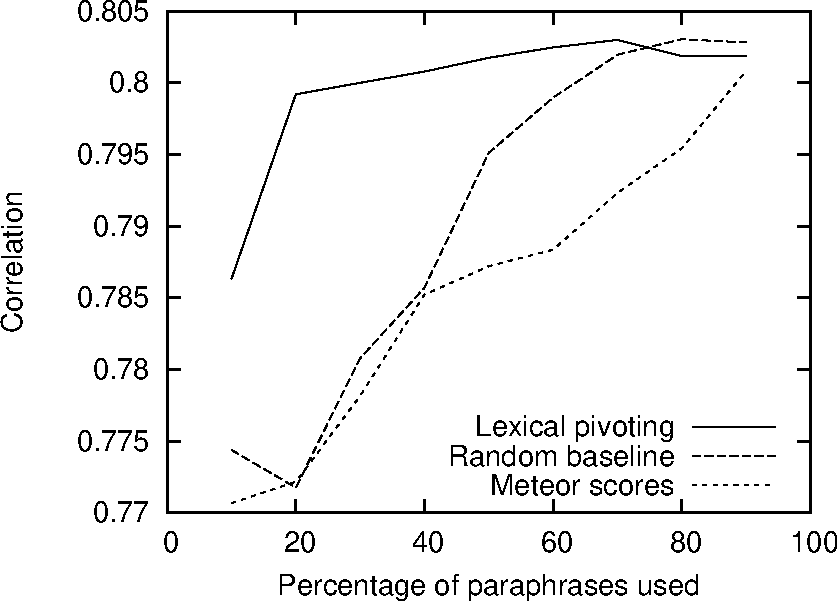
\includegraphics[scale=0.55]{../img/filtering-lexical-cropped.pdf}
\caption{Comparison of automatic filtering techniques for~\emph{one-word} paraphrases on WMT12 data.}
\label{fig:filtering-lexical}
\end{center}
\end{figure}

\begin{figure}[tb]
\begin{center}
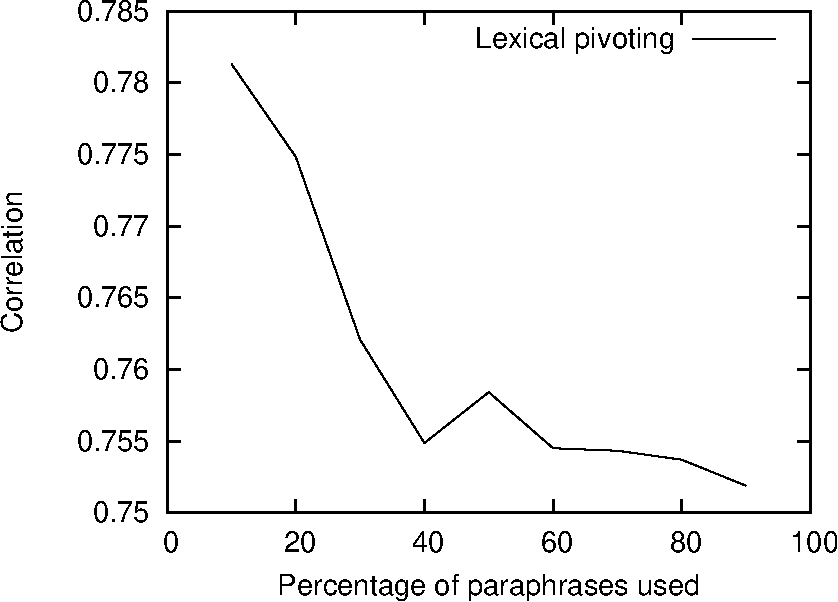
\includegraphics[scale=0.55]{../img/filtering-mwe-cropped.pdf}
\caption{Automatic filtering of multi-word paraphrase for~the \textit{multi-word-first} scenario on WMT12 data.}
\label{fig:filtering-mwe}
\end{center}
\end{figure}

\Fref{fig:filtering-lexical} shows the performance of different filtering techniques for one-word paraphrases. 
Relying on the Meteor scores proves worse than random selection. 
Using lexical pivoting, we can keep a high correlation even if we throw away as much as 80\% of the paraphrases, however we do not improve (by~a~relevant margin) upon the baseline correlation of 0.802 achieved by \emph{one-word-only} paraphrasing with the full paraphrase table.

We evaluate the best-performing technique also in the  \emph{multi-word-first} scenario where we use it for filtering multi-word paraphrases (see \Fref{fig:filtering-mwe}). 
As we reduce the number of paraphrases, we observe a considerable improvement of~correlation, however we never outperform \textit{one-word-only} or \textit{one-word-first}. 
In this case, the filtering simply mitigates the damage done by the multi-word paraphrases. 
%We cannot hope to achieve a higher score without a~more fine-grained grip on what a~good multi-word paraphrase is.


\subsection{PPDB} 